\section{Problem Description}\label{sec:prob_descr}

The system consists of an arm suspended on a base which can rotate freely around a vertical axis. On one end of the arm is the helicopter, consisting of two DC motors with rotor blades which are partially encased for safety. On the other end there is a counter weight which is adjusted so that the weight lifted from the motors are approximately 40g. A Quanser Q4 i used as a control board.


\begin{figure}[H]
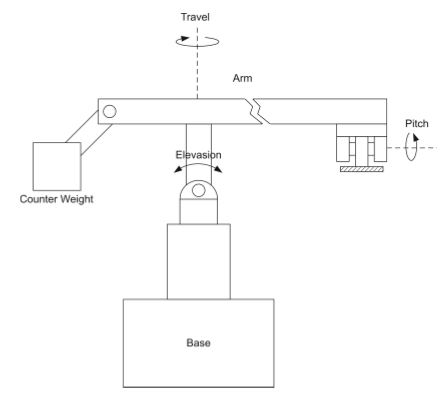
\includegraphics[width=1\linewidth, height=10cm]{figures/Helikopter.JPG}
\caption{The helikopter system}\label{fig:figur9}
\end{figure}

\newpage
\subsection{Model Derivation}\label{sec:mod_der}
A mathematical model for the system is derived from first principles. 

For elevation we have:

\begin{subequations}
\begin{equation}\label{eq:model_elevation1}
J_{e} \ddot{e} = l_{a} K_{f} V_{s} - T_{g}
\end{equation}

\begin{equation}\label{eq:model_elevation2}
\ddot{e} = K_{3} V_{s} - \frac{T_{g}}{J_{e}}\,\quad K_{3} = \frac{l_{a}K_{f}}{J_{e}}\
\end{equation}
\end{subequations}

The pitch is controlled by a PD controller and is modelled in the following way:

\begin{subequations}
\begin{equation}\label{eq:model_pitch1}
J_{p} \ddot{p} = l_{h} K_{f} V_{d}
\end{equation}

\begin{equation}\label{eq:model_pitch2}
\ddot{p} = K_{1} V_{d},\quad K_{1} = \frac{l_{h}K_{f}}{J_{p}}\
\end{equation}
\end{subequations}

The horizontal component of the force from the helicopter gives us the acceleration around the travel axis:

\begin{subequations}
\begin{equation}\label{eq:model_travel1}
\ddot{p} = -K_{p} l_{a} sin(p)
\end{equation}

\begin{equation}\label{eq:model_travel2}
\dot{r} = -K_{2}p,\quad K_{2} = \frac{l_{a}K_{p}}{J_{t}}\
\end{equation}
\end{subequations}

\newpage
\subsection{Assumptions, Limitations and the Final Model}
All controllers are assumed properly tuned in this project, and also that the motors output a force which is proportional to the voltage applied to them. The elevation is controlled by a PID controller and we assume that the constant term \(\frac{T_{g}}{J_{e}}\) is cancelled out by the integral term. We also assume that the pitch angle is small, such that the force to keep the helicopter flying is approximately \(K_{p}\) and \(\sin(p)=p\). This is not the case and will be a source of error. Taking these into account we end up with the final model:

\begin{subequations}\label{eq:model_al}
	\begin{align}
		\ddot{e} + K_{3} K_{ed} \dot{e} + K_{3} K_{ep} e &= K_{3} K_{ep} e_{c} \label{eq:model_se_al_elev} \\
		\ddot{p} + K_{1} K_{pd} \dot{p} + K_{1} K_{pp} p &= K_{1} K_{pp} p_{c} \label{eq:model_se_al_pitch} \\
		\dot{\lambda} &= r \label{eq:model_se_al_lambda} \\
		\dot{r} &= -K_{2} p \label{eq:model_se_al_r} 
	\end{align}
\end{subequations}

Parameters and variables are given in table 1 and 2.


\newpage
\begin{table}[tbp]
	\centering
	\caption{Parameters and values}
	\begin{tabular}{l1ll}
		\toprule
		Symbol & Parameter & Value & Unit \\
		\midrule
		$l_a$ & Distance from elevation axis to helicopter body & $0.63$ & \meter\\
		$l_h$ & Distance from pitch axis to motor & $0.18$ & \meter\\
		$K_f$ & Force constant motor & $0.25$ & \newton\per\volt\\
		$J_e$ & Moment of inertia for elevation & $0.83$ & \kilogram\usk\meter\squared\\
		$J_t$ & Moment of inertia for travel & $0.83$ & \kilogram\usk\meter\squared\\
		$J_p$ & Moment of inertia for pitch & $0.034$ & \kilogram\usk\meter\squared\\
		$m_h$ & Mass of helicopter & $1.05$ & \kilogram\\
		$m_w$ & Balance weight & $1.87$ & \kilogram\\
		$m_g$ & Effective mass of the helicopter & $0.05$ & \kilogram\\
		$K_p$ & Force to lift the helicopter from the ground & $0.49$ & \newton\\
		\bottomrule
	\end{tabular}
\label{tab:parameters}
\end{table}

\newpage
\begin{table}[tbv]
	\centering
	\caption{Variables}
	\begin{tabular}{l1ll}
		\toprule
		Symbol & Variable \\
		\midrule
		$p$ & Pitch \\
		$p_{c}$ & Setpoint for pitch\\
		$\lambda$ & Travel\\
		$r$ & Speed of travel\\
		$r_{c}$ & Setpoint for speed of travel\\
		$e$ & Elevation\\
		$e_{c}$ & Setpoint for elevation \\
		$V_{f}$ & Voltage, motor in front\\
		$V_{b}$ & Voltage, motor in back\\
		$V_{d}$ & Voltage difference, \(V_{f}-V_{b}\)\\
		$V_{s}$ & Voltage sum, \(V_{f}+V_{b}\)\\
		$K_{pp},K_{pd},K_{ed},K_{ei},K_{ed}$ & Controller gains\\
		$T_{g}$ & Moment needed to keep the helicopter flying\\
		\bottomrule
	\end{tabular}
\label{tab:parameters}
\end{table}
